\documentclass[a4paper,11pt]{article}
\usepackage{geometry}
\usepackage[utf8]{inputenc}
\usepackage{hyperref}
\usepackage{siunitx}
\DeclareSIUnit\barn{b}
\usepackage{amsmath}
\usepackage{graphicx}
\usepackage{subcaption}
\usepackage{biblatex}
\usepackage{fancyhdr}

\addbibresource{biblio.bib} 
\usepackage{mathptmx}


\geometry{a4paper, left=20mm, right=20mm, top=30mm, bottom=30mm}
\title{Report CMEPDA}
\author{Giulio Cordova \qquad Matilde Carminati}
\date{\today}

\begin{document}
\pagestyle{fancy}
\fancyhead{} % clear all header fields
\fancyhead[RO,LE]{\textbf{YCrossFit: A C++ Library for calculating the differential cross section in $p_T$ of $\Upsilon$(nS) states}}
\fancyfoot{} % clear all footer fields
\fancyfoot[LE,RO]{Report CMEPDA}
\fancyfoot[LO,CE]{Giulio Cordova, Matilde Carminati}
\fancyfoot[CO,RE]{\thepage}
\maketitle
\begin{abstract}
    A software able to cut a dataframe and fit lineshapes with customizable parameters was written in order to perform the analysis of the differential cross sections as a function of transverse momentum $p_T$ for the production of $\Upsilon$(nS) (n = 1, 2, 3) states decaying into a pair of muons. Data corresponding to an integrated luminosity of \SI{11.6}{\per\femto\barn} in pp collisions at $\sqrt{s} = \SI{8}{\tera\eV}$ were collected with the CMS detector at the LHC and acquired by us via the CMS Open Data portal. This analysis selects events with dimuon rapidity $|y| < 1.2$ and dimuon invariant mass in the range $8.5 < p_T < \SI{11.5}{\giga\eV}$, although these values are customizable in the software.

\end{abstract}
%\tableofcontents
\section{Introduction}
%vedere articolo
Hadronic production of S-wave bb mesons has been extensively studied for many years. 
%At the CERN LHC, the CMS, ATLAS and LHCb Collaborations have published results on $\Upsilon$(nS) (n = 1, 2, 3) production cross sections times dimuon branching fractions in pp collisions at $\sqrt(s)=7$ TeV as a function of the $\Upsilon$ transverse momentum, rapidity and polarization.
Measurements of S-wave bb mesons provide an important probe of quantum chromodynamics (QCD), since there are several models that predict differential cross section shapes at high $\Upsilon$(nS) $p_T$ in pp collisions, and all of them have contributing terms that vary with $p_T$.
A good description of early LHC results for $\Upsilon$(1S) production for $p_T < \SI{30}{\giga\eV}$ was achieved using nonrelativistic QCD (NRQCD) with next-to-leading-order (NLO) corrections. However, there are theoretical corrections to perturbative NRQCD that have characteristic power-law behavior at high $p_T$, and measurements at high $p_T$ (where different corrections become dominant) can help to clarify the theoretical picture. 

In this report we present a calculation of the differential production cross sections of the three lowest-mass $\Upsilon$(nS) states in pp collisions at $\sqrt{s}=\SI{8}{\tera\eV}$ up to $p_T = \SI{100}{\giga\eV}$. 
We plot the $p_T$ dependence of the $\Upsilon$(nS) differential cross section times the branching fraction to $\mu^+\mu^-$ using the DoubleMuParked dataset from 2012 in NanoAOD format reduced on muons\cite{dataA} from the CMS experiment, corresponding to an integrated luminosity of $\SI{11.6}{\per\femto\barn}$. 

The main focus in this project was to perform a data analysis with computationally efficient code and a software organization such that people reviewing or reusing the software could understand it easily. For this reason, some results may not result optimal.

\section{Differential cross section measurement methodology}
%vedere articolo
Event selection is done with a series of trigger on the presence of at least two high-energy muons in the event. More information about the Data taking and High-Level Trigger (HLT) can be found on the CERN open data platform \cite{dataB}\cite{dataC}.

This trigger selected dimuons in the invariant mass region spanning more than three orders of magnitude, from a few hundred MeV/$c^2$ to a few hundred GeV/$c^2$.
The following kinematic requirements are also imposed to ensure accurate muon detection efficiency evaluation:
\begin{align}
p_T(\mu) &> \SI{3}{\giga\eV} &   \text{ for } 1.4 < |\eta(\mu)|&< 1.6,\\\nonumber
p_T(\mu) &> \SI{3.5}{\giga\eV} &  \text{ for } 1.2< |\eta(\mu)|&<1.4,\\\nonumber
p_T(\mu) &> \SI{4.5}{\giga\eV} & \text{ for } |\eta(\mu)|&< 1.2.
\end{align}

The differential cross section is measured in the rapidity range $|y| < 1.2$. The data are binned in $p_T$, with bin edges at 2 GeV intervals between 12 and 40 GeV, then wider bins with edges at 43, 46, 50, 55, 60, 70, and 100 GeV.
The $\Upsilon(nS)$ differential cross section times dimuon branching fraction, integrated over either of the two $|y|$ ranges and in a given $p_T$ bin of width $\Delta p_T$, is
\begin{equation}
\left.\frac{\mathrm{d} \sigma(\mathrm{pp} \rightarrow \Upsilon(n \mathrm{~S}))}{\mathrm{d} p_{\mathrm{T}}}\right|_{|y| \text { range }} \mathcal{B}\left(\Upsilon(n \mathrm{~S}) \rightarrow \mu^{+} \mu^{-}\right)=\frac{N_{\Upsilon(n \mathrm{~S})}^{\mathrm{fit}}\left(p_{\mathrm{T}}\right)}{L \Delta p_{\mathrm{T}} \epsilon_{\mu \mu}\left(p_{\mathrm{T}}\right) \mathcal{A}\left(p_{\mathrm{T}}\right) \epsilon_{\mathrm{sg}} \epsilon_{\mathrm{vp}}}\end{equation} 
where $N^{fit}_{\Upsilon(nS)}$ is the fitted number of $\Upsilon$(nS) events from the dimuon invariant mass distribution in a $p_T$ bin for the selected $|y|$ range, $\epsilon_{\mu\mu}$ is the dimuon efficiency, L is the integrated luminosity, $\mathcal{A}$ is the polarization-corrected acceptance, $\epsilon_{sg}$ is the efficiency of the seagull selection, and $\epsilon_{vp}$ is the efficiency of the dimuon vertex $\chi ^2$ probability requirement. The efficiency and acceptance determinations are described below.

\subsection{Efficiency factors and acceptance}
%come avevamo scritto prima ma inserendo i valiri usati 
Since we did not have the Monte Carlo data to compute the efficiencies and the acceptance, we have taken the values reported in the article of reference:
\begin{itemize}
    \item $\epsilon_{\mu\mu} = 0.75$
    \item $\epsilon_{sg}  = 0.5$
    \item $\epsilon_{vp} = 0.99$
\end{itemize}

These values represent an average of the efficiencies. In the reality, this ones vary with the binning in $p_T$.

The values of acceptance for each $p_T$ bin and $\Upsilon$ state can be found in the Tables A.9, A.12, A.15 of the appendix A of the article of reference \cite{Khachatryan_2015}.

\section{Fitting}
%grafici fit alle risonanze senza tagli e un grafico con i talgi di un bin con i risultati del fit
The $\Upsilon$(nS) lineshape for a given $p_T$ bin is expressed by a probability density function (PDF) for the signal dimuon mass $M_{\mu\mu}$. For this project, it was decided to use a gaussian distribution
\begin{equation}
    F(M_{\mu\mu};m,\sigma)=\frac{1}{\sqrt{2\pi \sigma}} \exp\biggl(-\frac{(M_{\mu\mu}-m)^2}{\sigma^2}\biggr)
\end{equation}
where $m$ is the mass of the resonance and $\sigma$ its width. 
The background was modeled with a second degree polynomial, leading to define a model for the complete unnormalized PDF:
\begin{equation}\label{model}
    P(M_{\mu\mu};N_n,m_n,\sigma_n,a_0,a_1,a_2)=
    \sum_{n=1}^3 \frac{N_n}{\sqrt{2\pi \sigma_n}} \exp\biggl(-\frac{(M_{\mu\mu}-m_n)^2}{\sigma_n^2}\biggr)+(a_0+a_1M_{\mu\mu}+a_2M_{\mu\mu}^2)N_{back}
\end{equation}
where the index n refers to the three $\Upsilon$(nS) resonances and $N_n$ to the total number of events yield under each curve. We measure them by performing an extended maximum-likelihood estimation (MLE) fit using $\text{RooFit}$ to determine the number of signal events associated with each normalized signal PDF. 

\begin{figure}[h]
    \centering
    \begin{subfigure}{.49\textwidth}
    \centering
    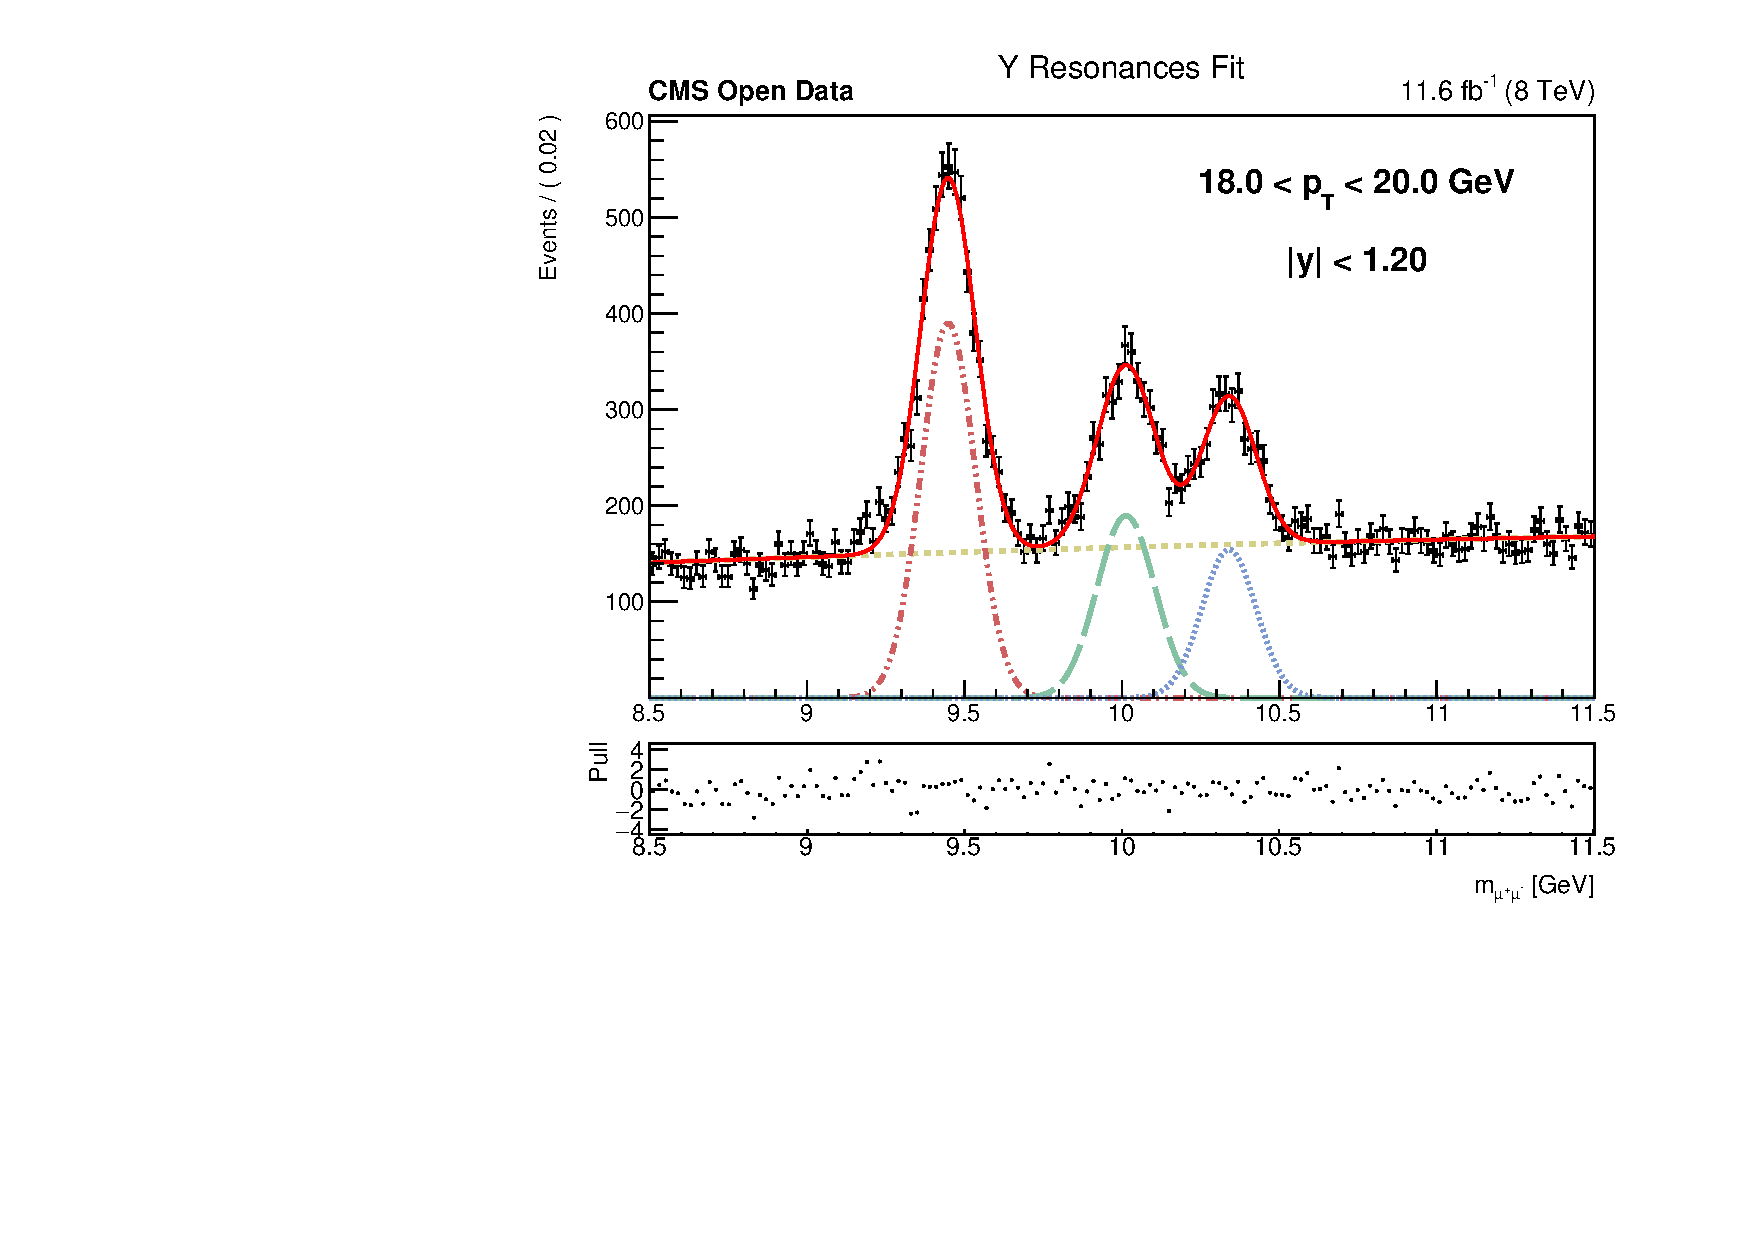
\includegraphics[width=\textwidth]{YResonances_3.pdf}
    \end{subfigure}
    \begin{subfigure}{.49\textwidth}
  \centering
    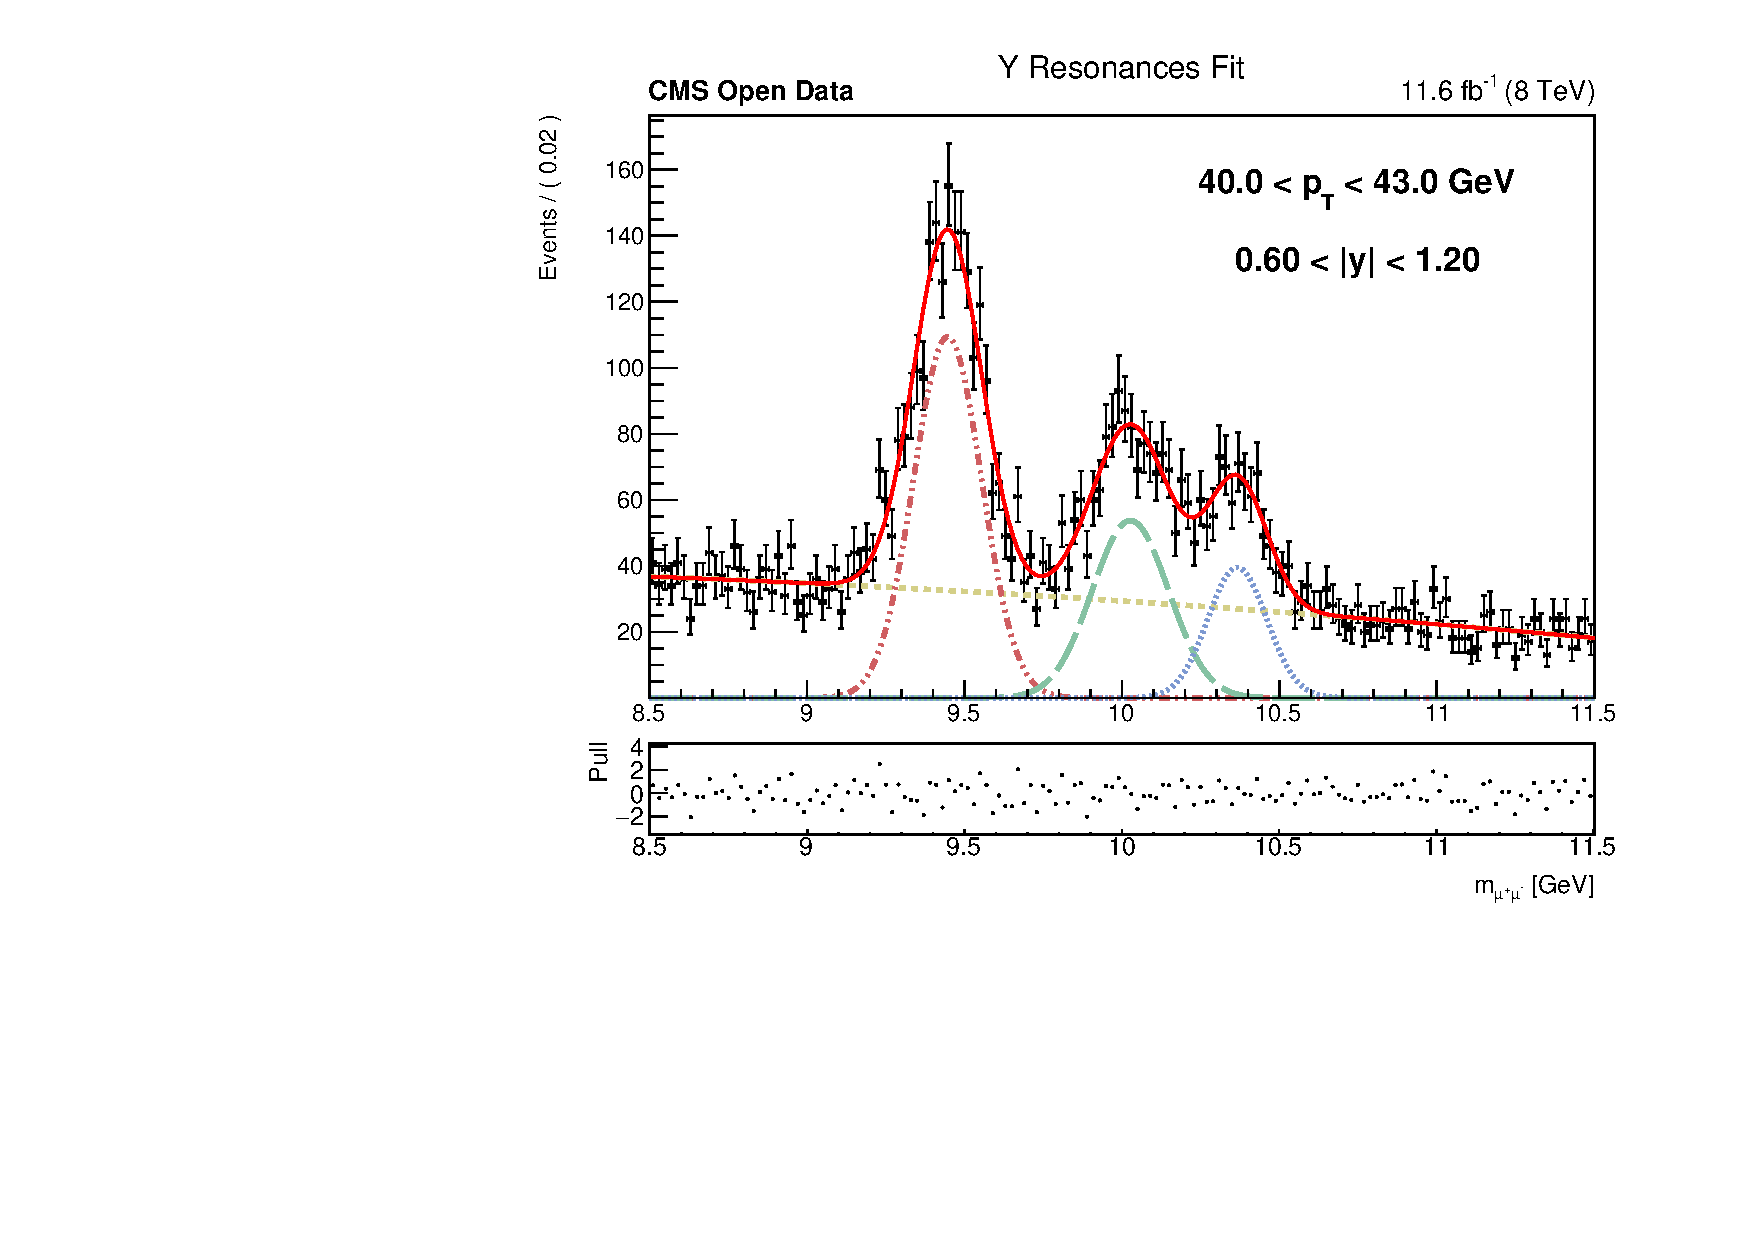
\includegraphics[width=\textwidth]{YResonancesFit.pdf}
    \end{subfigure}
    \caption{Results of the fits to the dimuon invariant mass distribution for events in two bins.The solid line is the result of the full fit. The dash-dotted line is the $\Upsilon$(1S) signal fit, the long-dashed line is the $\Upsilon$(2S) signal fit, and the dotted line is the $\Upsilon$(3S) signal fit. The short-dashed line is the background contribution. The lower plots show the pull for each mass bin.}
    \label{fig:fit}
\end{figure}%

\begin{table}[!h]
    \centering
    \begin{subtable}{.43\linewidth}
    \bgroup
    \def\arraystretch{1.2}
    \resizebox{\textwidth}{!}{%
    \begin{tabular}{c|c|c}
 Floating Parameter & InitialValue  &  FinalValue $\pm$  Error  \\
\hline
                    a0  &   $50.473$   & $(1.0510 \pm  0.314)$$10^3$  \\
                    a1  &   $10.403$   & $5.3018 \pm  13.4$  \\
                    a2  &   $0.0$      & $-2.1123 \pm  0.796$  \\
                 mass1  &   $9.45$     & $ (9448.5 \pm  2.10)$$10^{-3}$ \\
                 mass2  &   $10.01$    & $ (10013 \pm  4.31)$ $10^{-3}$\\
                 mass3  &   $10.35$    & $ (10340 \pm  5.03)$$10^{-3}$ \\
                 nback  &  $10.063$$10^3$  & $ (23.372 \pm  0.206)$ $10^3$\\
                 nsig1  &  $13.208$$10^3$  & $ 4223.6 \pm  99.6$  \\
                 nsig2  &  $9.7489$$10^3$  & $ 2189.4 \pm  96.21$  \\
                 nsig3  &  $6.9186$$10^3$  & $ 1663.5 \pm  89.3$  \\
                sigma1  &  $54.0$$10^{-3}$    & $ (86.384 \pm  2.22)$ $10^{-3}$\\
                sigma2  &  $32.0$$10^{-3}$    & $ (92.120 \pm  4.79)$$10^{-3}$ \\
                sigma3  &  $20.0$$10^{-3}$    & $ (85.961 \pm  5.26)$$10^{-3}$ \\
    \end{tabular}%
    }%
    \egroup
    \caption{$18<p_T<\SI{20}{\giga\eV}$ and $|y|<1.2$}
    \label{tab:fig1}
    \end{subtable}%
    \hfil%
    \begin{subtable}{.47\linewidth}
            \bgroup
    \def\arraystretch{1.2}
    \resizebox{\textwidth}{!}{%
    \begin{tabular}{c|c|c}
 Floating Parameter & InitialValue  &  FinalValue $\pm $ Error  \\
\hline
                    a0  &   $109.54$   &  $103.14 \pm  4.65$  \\
                    a1  & $-8.0537$    & $-8.5644 \pm  0.376$  \\
                    a2  &   $0.0$   &  $(60.104e-02 \pm  31.0)$$10^{-3}$  \\
                 mass1  &  $9.4500$    &  $(9446.9 \pm  4.19)$$10^{-3}$  \\
                 mass2  &  $10.010$    &  $(10027 \pm  11.0)$$10^{-3}$  \\
                 mass3  &  $10.350$    &  $(10367 \pm  12.4)$$10^{-3}$ \\
                 nback  &  $2.2605$$10^3$  &  $4306.4 \pm  94.9$  \\
                 nsig1  &  $2.9669$$10^3$  &  $1479.0 \pm  55.8$  \\
                 nsig2  &  $2.1898$$10^3$  &  $816.15 \pm  63.8$  \\
                 nsig3  &  $1.5541$$10^3$  &  $462.73 \pm  58.4$  \\
                sigma1  &  $54.0$$10^{-3}$    &  $(107.87 \pm  4.17)$$10^{-3}$  \\
                sigma2  &  $32.0$$10^{-3}$    &  $(121.26 \pm  10.7)$$10^{-3}$  \\
                sigma3  &  $20.0$$10^{-3}$    &  $(93.459 \pm  12.3)$$10^{-3}$  \\
    \end{tabular}%
    }
    \egroup%
    \caption{$40<p_T<\SI{43}{\giga\eV}$ and $0.6<|y|<1.2$}
    \label{tab:fig2}
    \end{subtable}
    \caption{Results returned by RooFit for the fit in the two bins, with respect to the initialized parameters. These parameters relies on the model PDF defined in Eq. \eqref{model}. The initial value of the mass and the sigma are the same for every fit in each binning, while the initial parameters relative to the background polynomial depend on the $p_t$ binning. The $Nsig_n$ (n=1,2,3) parameters are extracted in each fit for computing the differential cross sections.}
\end{table}


For the initialisation of the signal fit parameters, such as the $\Upsilon$ masses and widths, we take the values from the Particle Data Group. Furthermore, the initial parameters for the background function are chosen by computing a slope using the extreme points of the histogram, while the offset is set accordingly to the slope. The curvature is initialized to zero.

The plots in Fig. \ref{fig:fit} show two examples of fitting the dimuon invariant mass distribution. The lower plots show the pull, $(N_{data} - N_{fit})/\sigma_{data}$, in each dimuon mass bin, where $N_{data}$ is the observed number of events in the bin, $N_{fit}$ is the integral of the fitted signal and background function in that bin, and the uncertainty $\sigma$ data is the Poisson statistical uncertainty. As example, the results returned by RooFit for the fit in the two bins, with respect to the initialized parameters, are also reported in the Table \ref{tab:fig2}. 

\section{Results}
%grafico sezione d'urto differenziale
The measured $\Upsilon$(nS) differential cross sections versus $p_T$ are shown in Fig. \ref{fig:diffcrosssec} over the full rapidity range $|y| < 1.2$. The vertical bars on the points in Fig. \ref{fig:diffcrosssec} show the statistical uncertainties.
\begin{figure}[h]
    \centering
    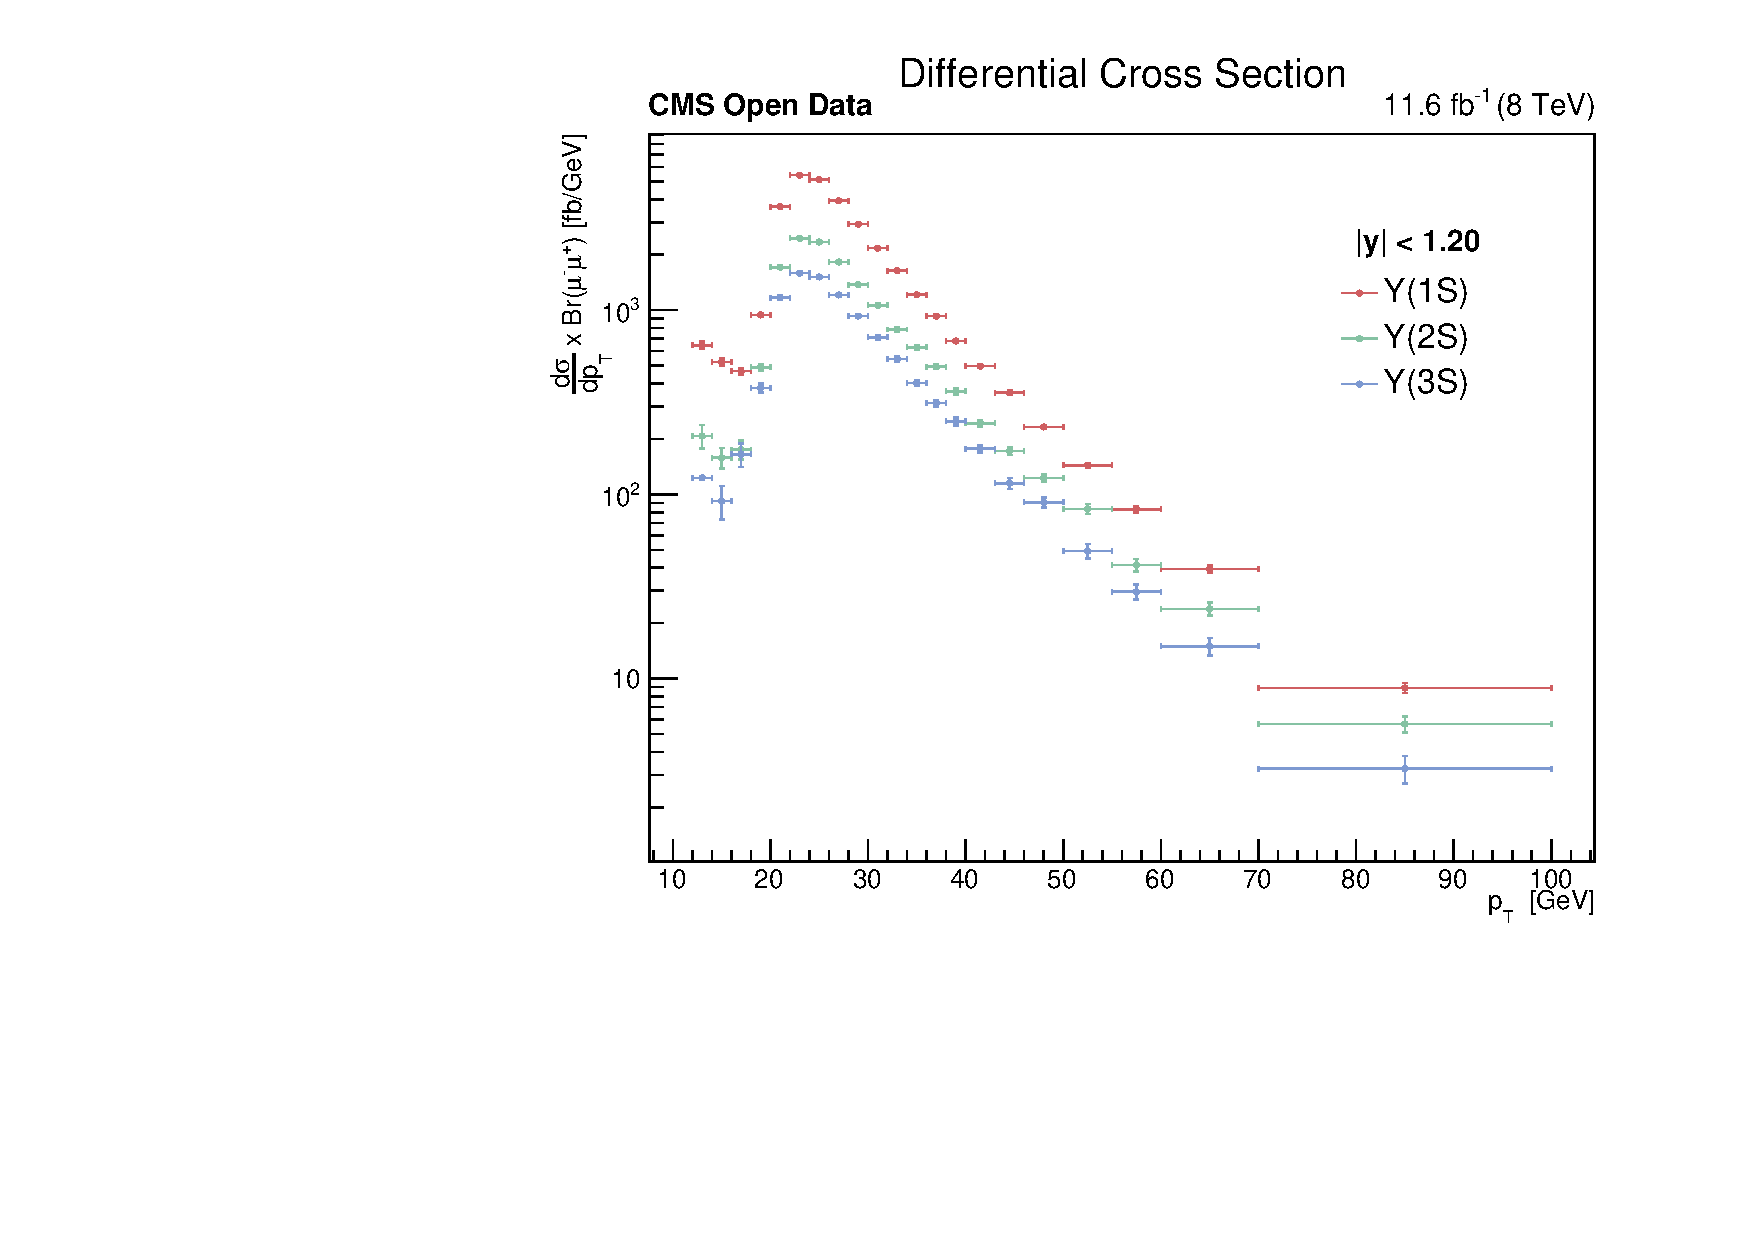
\includegraphics[width=0.5\textwidth]{diffCrossSection.pdf}
    \caption{The $\Upsilon$(nS) differential $p_T$ cross sections times dimuon branching fractions for $|y| < 1.2$. The vertical bars show the total uncertainty, excluding the systematic uncertainty in the integrated luminosity. The horizontal bars show the bin widths.}
    \label{fig:diffcrosssec}
\end{figure}

Looking at Figure \ref{fig:diffcrosssec}, we observe two different behaviour, at low and high energy. At high energy, the trend looks like an exponential, while at the low scale is not well-defined. 
Comparing our result with the CMS one\cite{Khachatryan_2015}, it is visible the effect of the two different behaviour does not exist. One of the possible explanation may rely on the fact that we have used average efficiency factors for all the bins.
We also notice an evident difference in the y axis scale of a factor $10^2$ for the bins at high energy. 

A possible further development could be the fitting of the differential cross sections with exponential and power-law parametrisation such as
\begin{equation}
    \left.\frac{\mathrm{d} \sigma(\mathrm{pp} \rightarrow \mathrm{Y}(n \mathrm{~S}))}{\mathrm{d} p_{\mathrm{T}}}\right|_{|y| \text { range }} \mathcal{B}\left(\mathrm{Y}(n \mathrm{~S}) \rightarrow \mu^{+} \mu^{-}\right)=\frac{A}{C+\left(\frac{p_{\mathrm{T}}}{p_0}\right)^\alpha},
\end{equation}
in order to investigate the NRQCD + NLO predictions.

\section{Summary of the analysis}
Measurements of the differential production cross sections as a function of $p_T$ for the $\Upsilon$(1S), $\Upsilon$(2S), and $\Upsilon$(3S) states in pp collisions at $\sqrt{s} = \SI{8}{\tera\eV}$ have been presented, based on a data sample corresponding to an integrated luminosity of \SI{11.6}{\per\femto\barn} collected by the CMS experiment at the LHC. It was not possible to investigate the power-law nature of the $p_T$ distributions for all three $\Upsilon$(nS) states at high $p_T$ due to an incomplete access of the Monte Carlo data for determining the acceptance and efficiencies for these data.

\newpage

\section{Software description}
\subsection{Functionalities of the YCrossFit library}
In this section a brief description of the program functionalities and its implementation is provided. This is not a documentation page, so there will not be details. For a more accurate description of the code, please refer to the \href{https://zenith378.github.io/Y-DiMuonResonances/html/index.html}{documentation page}.

We can summarize the workflow of the program in the following steps:
\begin{itemize}
    \item set flag and options
    \item read data (and wisely store it, if not already present locally)
    \item apply some user-defined cuts (optional)
    \item create an histogram of the invariant mass
    \item resolve and fit the upsilon states
    \item calculate and plot the differential cross sections in $p_T$
\end{itemize}

\subsubsection{Flags and Options}
A function handling command line arguments as flags or options was necessary. For example, an option [\texttt{--mode}] was implemented for deciding whether to just fit the dataset, or to plot the differential cross section in $p_T$. Another flag was necessary to select the PDF used to perform the fit [\texttt{--fitFunction}], or another one to show the output of MINUIT during the MLE fit [\texttt{--verbose}]. A comprehensive list of the flags and their functionalities can be seen  \href{https://zenith378.github.io/Y-DiMuonResonances/html/optionParse_8h.html#ae964ff8411b4fdcaf65cb5529aea4bef}{in the documentation} or just by using the flag \texttt{--help}.

The acquisition of these parameters from the command line was implemented with the help of the library \href{https://man7.org/linux/man-pages/man3/getopt.3.html}{getopt}.

In the file optionParse.C are also defined some functions in order to handle out of boundaries values or incorrect types.

\subsubsection{Data reading (and writing)}
We used a CMS open dataset in this analysis. The reading of the online dataset is quite a long task (up to 25 minutes, depending on the internet connection). For this reason, it was decided to store the data in an RDataFrame and save it a root file with a Snapshot().


It was decided to implement a function that checks for the existence of the data.root file in the folder Data. If they are not present, the function creates them.

Before storing the data in the file, it was decided to modify the dataframe in order to discard uninteresting events (to reduce the size of the file) and to define useful variables in the upcoming tasks.

First, single muons were kept that satisfied the kinematics constrains defined in the Equation 1 of the article of reference. The dataset were then filtered for keeping only at least two muons of opposite charge, and a PtEtaPhiMass four-vector was computed as the sum of the two muons four-vector. New columns were defined, such as the pt, rapidity, beta and mass of the dimuon four vector just created. Lastly, a cut around on the invariant mass is performed, to limit the dataset in upsilon region (between $8.5$ and $11.5$ GeV).

 TheRDataFrame container resulted pretty helpful in this task because of its useful properties, such as declarative analysis, multi-threading and other low-level optimisations that allow users to exploit all the resources available on their machines completely transparently.
 
\subsubsection{Cuts}
It is possible to choose custom cuts on the transverse momentum and the rapidity of the dimuon state, by adding the appropriate options while calling the program from the terminal. This is useful for performing a fit with custom cuts. This feature is also used in the differential cross section calculation, because it loops over the fit with different values of $p_T$.
For filtering the dataset, decalrative analysis was used in order to apply the cuts. This is possible because of the just-in-time compilation.

\subsubsection{Spectrum plot}
A preliminary histogram of the invariant mass of the dimuon is created by using the method Histo1D of RDataFrame. The histogram is plotted in a canvas, which is then saved in the folder Plots. If the folder Plots does not exist, the program automatically creates it. The saved plot could be useful for checking the consistence of the performed fit. The histogram is then saved in a TH1 container since it is easier to store it in a RooDataHist.

\subsubsection{Fit plot}\label{fit}
For fitting the histogram created in the previous step, we used the package RooFit, a toolkit for modeling the expected distribution of events by performing an unbinned maximum likelihood fit. The advantage of this library is to define a model fit PDF with different components whose fit results are easily separately accessible. In particular we found useful the result that indicate how many events are counted under a certain component as we needed for the calculation of the differential cross section. 
If the fit result does not satisfy certain conditions on the convergence and estimated distance to minimum, the program exit with a fit error code and the result is not displayed.
The data and the fitted function are plotted in a canvas that is then saved in the folder Plots. The canvas is shown interactively thanks to a TApplication, if the flag [\texttt{--muteCanvas}] is not used.

\subsubsection{Differential cross section}
The differential cross section in $p_T$ is calculated with the same binning and parameters (efficiencies, etc.) of the article of reference. The acceptance was considered equal to one, because we did not have the Monte Carlo data for estimating it in each $p_T$ bin. 
To calculate the differential cross section, we need the number of events, which are the area under each shape of the resonances, for each bin in $p_T$. In order to get this quantity, we loop over the bin edges, cutting the dataframe according to them, and performing a fit as defined in Section \ref{fit}. The area under each resonance is used to calculate the differential cross section, which is then saved in a structure with its associated uncertainty. This structure is finally used to plot a multigraph of the differential cross sections of the three $\Upsilon$ resonances.

\subsection{Coding Style Options}
The styling of the code files is formatted and checked using the library clang-format, using the guidelines provided by the ROOT official page.

\subsection{Shared Library Implementation}
This project was built with \href{https://cmake.org}{CMake}, "an open-source, cross-platform family of tools designed to build, test and package software. CMake is used to control the software compilation process using simple platform and compiler independent configuration files, and generate native makefiles and workspaces that can be used in the compiler environment of your choice."
We found this platform really useful for keeping an organised project and implementing our shared library \textit{YCrossFit}, combining our code with the ROOT package.

\subsection{Testing}
CMake is also useful for defining unit testing for our library, using the command \texttt{ctest}, that automatically build targets for the tests. 
We chose to implement tests only on the functions created by us, instead of testing the functionalities of the ROOT library.

\paragraph{Test0} This test handles the reading of the command arguments and flags. In this test one define some variables, call the processArgs() and sees if the definition stands, then one modify the arguments and check if the options are evolved according to the made changes

\paragraph{Test1} Here is tested the online reading of the data and the behavior in case the Data folder or the Data file is missing. In the test, the folder Data is deleted and the function df\_set() is called. This function should handle the creation of the folder Data and the downloading and saving of the data. Once finished this first step, we check if the Data folder exists and if it contains the file data.root. Next, we keep the folder Data and we eliminate the file data.root. The function df\_set() is called again and after it finished, one check if the data is successfully recreated.

\paragraph{Test2}In this test the fit results are controlled. First off, one defines a model with a similar shape to the one expected and calls the function fitRoo() passing this model as an argument instead of the real data. The test checks if the fit converged by looking at the fitStatus and also check if the returned parameters are inside 5 sigma of the initial value.

\paragraph{Test3} This one tests the function SavePlot() which handles the saving of a canvas with a specific filename. If the folder Plots does not exist, it creates it.

\paragraph{Test4} This test is useful to check if the printing of the custom cuts on the canvas work. It compares the strings returned by the function formatYString() or formatPtString() with the expected ones.

\subsection{Documentation}
In order to write the documentation, we relied on the \href{https://www.doxygen.nl}{Doxygen} tool. The special comments for the documentation are written only in the header files, for avoiding a difficult read of the source code. In the header file, each function is declared and its functionality is described in this special code above the function declaration.
The source code is also well commented in order to guarantee a deeper understanding of the code. 

A doxyfile was written for generating the documentation in html format starting from the special comments in the source code. For a better understanding, a website mainpage was also created in order to explain the project with examples on the functionalities. It is more or less an "hands-on" guide for the library usage.

A continuous integration for the documentation is implemented by using the GitHub action \href{https://github.com/langroodi/doxygenize}{doxygenize} developed by langroodi. The output files are saved in a different branch than the code for the correct creation of the gh-page for the documentation.

\subsection{Future Developments}
Our code is not perfect. We tried implementing a library with as many useful functionalities as possible as we could in these two months of work. There are many possible ways of improving the code. Some are summarized in this list below:
\begin{itemize}
    \item Implementing environmental variables for accessing data and plots. Our code download the data again if they are not placed in the right relative path.
    \item Implementing some concurrential/parallel programming for some functions, e.g. the multiple fits over the bins for the computation of the differential cross section
    \item Implementing an installation, making possible running the program from anywhere in the terminal (including downloading the requirements)
    \item Implementation of more PDFs to fit the data (crystall ball, etc...)
    \item Implementation of the calculation of efficiencies and acceptance with a Monte Carlo
\end{itemize}

\printbibliography

\end{document}